\documentclass[]{thesis-ekf}
\usepackage[T1]{fontenc}
\PassOptionsToPackage{defaults=hu-min}{magyar.ldf}
\usepackage[magyar]{babel}
\usepackage{mathtools,amssymb,amsthm,pdfpages,listingsutf8,hyperref,url}
\footnotestyle{rule=fourth}

\newtheorem{tetel}{Tétel}[chapter]
\theoremstyle{definition}
\newtheorem{definicio}[tetel]{Definíció}
\theoremstyle{remark}
\newtheorem{megjegyzes}[tetel]{Megjegyzés}

\begin{document}
	\institute{Matematikai és Informatikai Intézet}
	\title{Adatbázis alapú web alkalmazás fejlesztése}
	\author{Verebélyi Valentin\\Programtervező Informatikus BSc}
	\supervisor{Dr.~Tajti Tibor Gábor\\Egyetemi Docens}
	\city{Eger}
	\date{2024}
	\maketitle
	\tableofcontents
	
	\chapter*{Bevezetés}
	\addcontentsline{toc}{chapter}{Bevezetés}
	
	\chapter{Tervezés}
		A tervezés egy nagyon fontos szerepet tölt be egy szoftvereknél. Az én meglátásom és tudásom szerint a következő okok miatt szükséges tervezni:
		\begin{enumerate}
			\item Tervezési célok meghatározása: fontos az, hogy mind a fejlesztő, mind a megrendelő egyértelműen megértse, hogy pontosan mit kell elérni a szoftverrel.
			\item Költség- és időmegtakarítás: implementálás előtt, ha kellő alapossággal tervezzük meg a szoftvert, akkor segíthet kiszűrni a későbbi fázisokban esetleges előforduló hibákat. 
			\item Bővíthetőség: ez alatt azt értem, hogy a szoftver úgy kell megtervezni, hogy fel legyen készítve arra, hogy lehessen hozzáadni könnyedén új funkciókat.
			\item Funkciók és feladatok felosztása: ez azért lehet hasznos, mivel a fejlesztés során a fejlesztők pontosan csak az ő általuk elvállalt feladatokat valósítják meg.
			\item Kommunikáció segítése: ha van egy jól kidolgozott terv, akkor ha a fejlesztők elakadnak valamiben vagy nem értik meg pontosan, hogy mit és hogyan kell implementálni, akkor elég, ha megnézik a tervben az adott dologhoz kapcsolódó részeket és ezáltal megtudják oldani a rájuk bízott feladatot.
		\end{enumerate}
	\section{A tervezéshez alkalmazott eszközök és technológiák}
		A következő alszakaszokban a tervezéshez használt eszközökről és technológiákról lesz majd szó.
	\subsection{Dbdiagram}
	A dbdiagram segítségével van lehetőség arra, hogy egy alkalmazás adatbázisának a sémáját és struktúráját megtervezzük és ehhez ad egy vizuális képet számunkra. A DBML-t, azaz Database Markup Language használja, amit magyarul talán adatbázis jelölőnyelvként tudnék lefordítani. Amiért a véleményem szerint nagyon hasznos még az nem más, mint, hogy rengetegféle olyan opciót ad számunkra, amire szükségünk lehet. Ilyen opciók például azok, hogy van lehetőség importálni be kódot MySQL, PostgreSQL, Rails valamint SQL szerverről. Ugyanezeket a típusú kódokat kilehet exportálni az imént megemlített típusokba, kivéve a Rails, mivel oda nem lehetséges. Ezenkívül van még olyan opció is, hogy ki lehet exportálni PNG, SVG vagy akár PDF formátumba is az elkészült tervet. A dbdiagram alap változata ingyenesen használható mindenki számára. \cite{Dbdiagram}
	
	A következőkben \aref{dbdiagram} képen látható adatbázisterv kódjáról szeretnék egy keveset még írni, pontosabban arról, hogy hogyan épül fel az előbb bemutatott terv. Csak a tervről mutatott be pár részletet az érdekesség kedvéért.
	
	\begin{figure}[ht!]
		\centering
		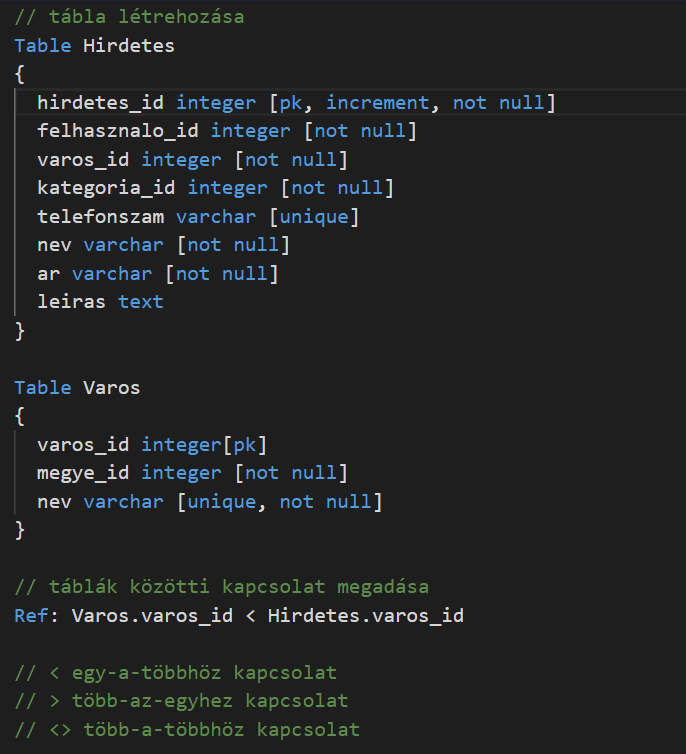
\includegraphics[width=10cm]{./tervezes/dbKod}
		\caption{DMBL kód részlet (Saját készítés)} 
		\label{dbKod}
	\end{figure}
	
	\Aref{dbdiagram} képen látható a dbdiagram-ban készített ábra az alkalmazásomhoz.
	
	\begin{figure}[ht!]
		\centering
		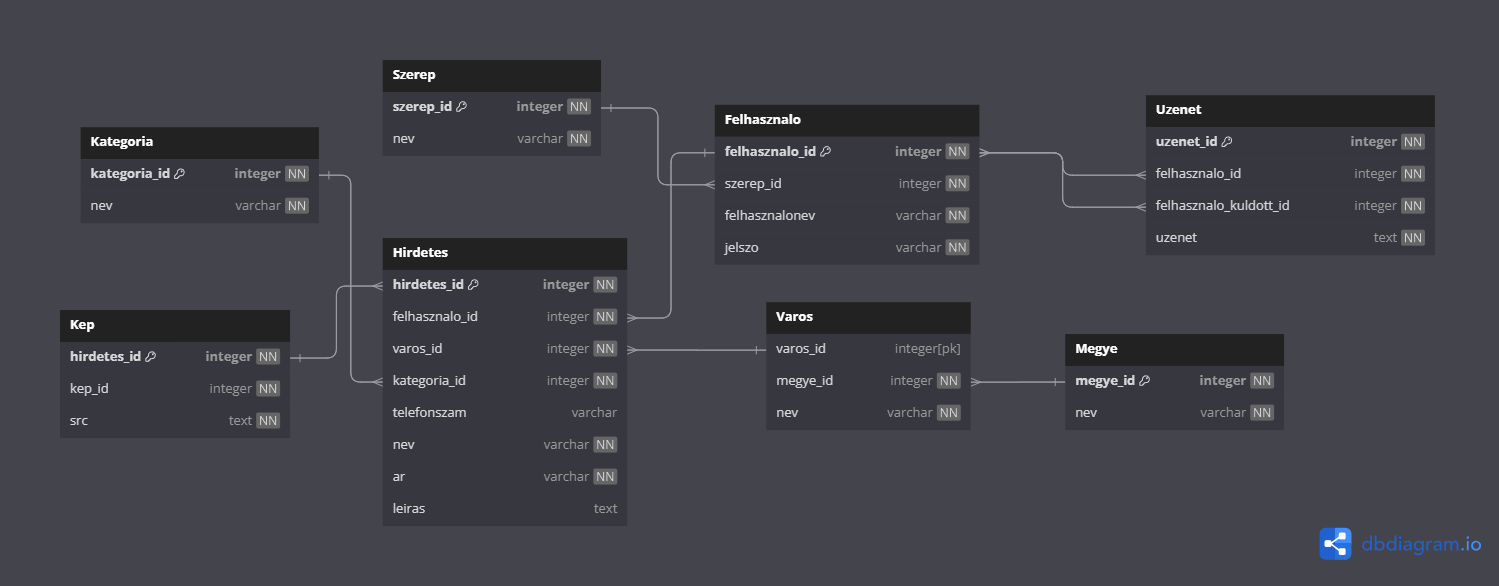
\includegraphics[width=15cm]{./tervezes/dbdiagram}
		\caption{Adatbázisterv (Saját készítés)} 
		\label{dbdiagram}
	\end{figure}
	
	\subsection{PlantUML}
	Az UML a Unified Modeling Language rövidítése, azaz Egységes Modellezési Nyelv. Az UML arra jó, hogy szoftvert tervezzünk vele, a gondolataimat letudom vele rajzolni, skiccelni. Ezenkívül a kiforrott megoldások dokumentálására is használható. A PlantUML egy komponens, aminek a segítségével gyorsan tudunk létrehozni szekvencia-, használati eset- és osztálydiagramokat. Ezenkívül még rengetegféle diagramot tudunk készíteni. \cite{PlantUML}
	
	Manapság a tervezés az használati eset központú. A következő pár mondatban az ilyenféle alapú tervezésről lesz szó. Tulajdonképpen itt azt a kérdést tehetjük fel, hogy ki (angolul: actor) mire (funkció) tudja használni az adott informatika rendszert. Az actor-ról azt érdemes tudni, hogy ő nem része az informatikai rendszernek, hame ő csak használja azt. Az actor gyakran lehet ember, AI vagy akár egy másik informatikai rendszer. Fontos az is, hogy minden ábra, amit készítünk az visszavezethető legyen a már meghatározott követelmények szintjéig. Az használati alapú tervezés előnye az, hogy egyszerűen, érthetően írja le a rendszer funkcióit. Ebből kifolyólag, mind a megrendelő, mind a tervező számára könnyen érthető az ábra. Tulajdonképpen a használati eset alapú tervezés nem más, mint egy közös nyelv a megrendelő és a tervező között, amit mind a két fél ért.\cite{Kusper Informatikai} \Aref{useCase} képen látható a plantUML-ben készített használati eset ábra az alkalmazásomhoz.
	\begin{figure}[ht!]
		\centering
		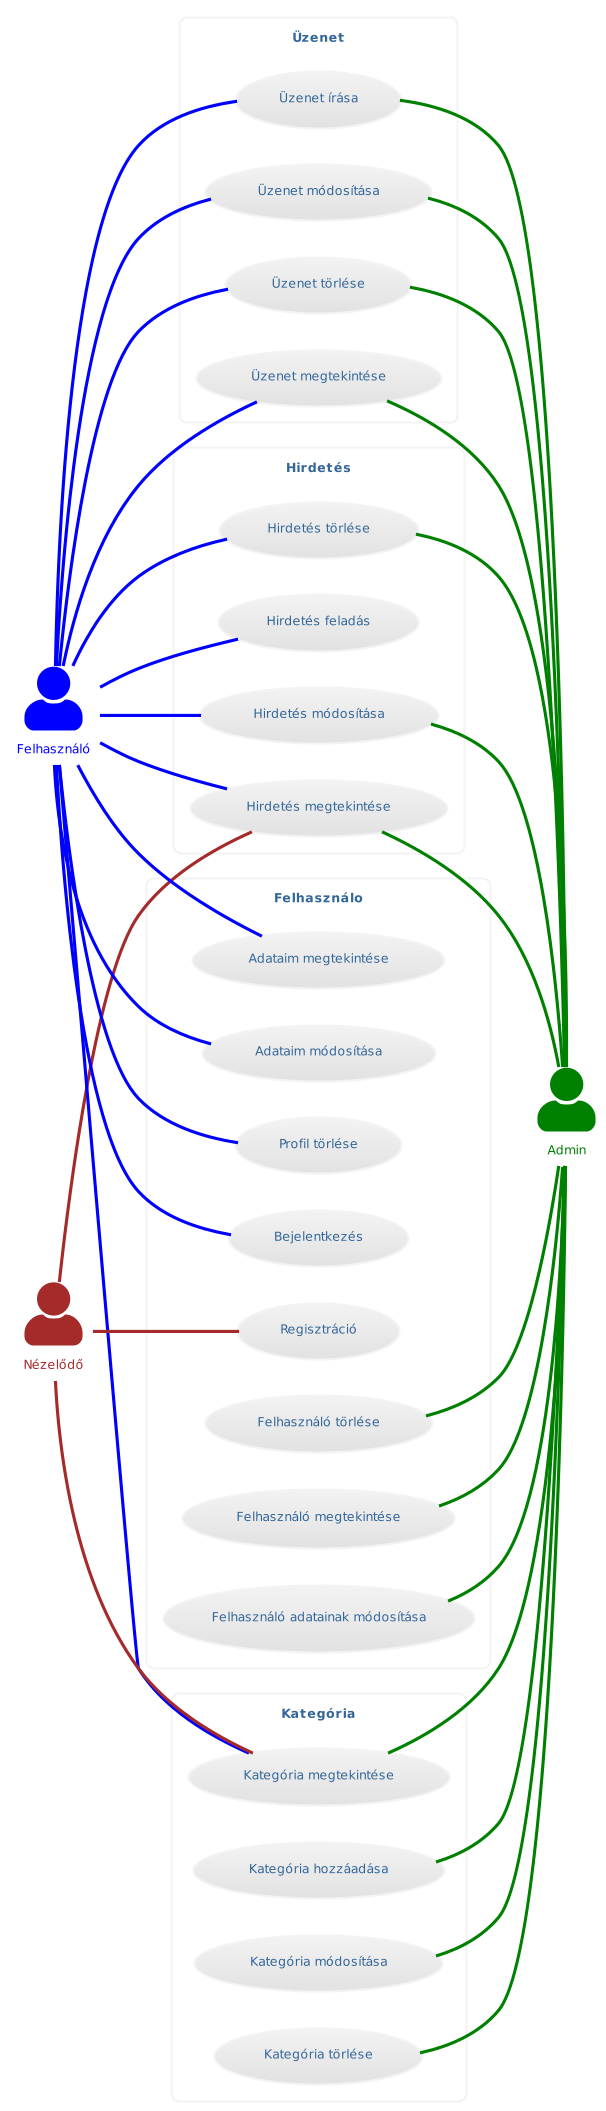
\includegraphics[width=6cm]{./tervezes/useCase}
		\caption{Használati eset (Saját készítés)} 
		\label{useCase}
	\end{figure}
	\Aref{useCase} képen látható használati eset ábra magyarázata következik:
	Az ábrán három darab actor látható.
	\begin{enumerate}
		\item Nézelődő: ennek a szerepnek van a legkevesebb funkciója, ő az aki csak a már meglévő hirdetéseket és kategóriákat tudja megtekinteni, illetve képes még regisztráció, ami további meglévő funkciók használata miatt szükséges.
		\item Felhasználó: ő képes a saját adatainak módosítására, a profil törlése is. Neki van már lehetősége saját hirdetéseket létrehozni és ezeket kezelni, valamint már van lehetősége üzenetet küldeni egy másik felhasználónak.
		\item Admin: neki már van lehetősége a kategóriákkal kapcsolatos műveletek elvégésére is. Szintén képes üzenetet küldeni bárkinek, ő képes már felhasználókat és hirdetések törölni az adott esetben.
	\end{enumerate}	

	\chapter{Fejlesztés}		
	\section{A fejlesztéshez alkalmazott eszközök és technológiák}
		A következő alszakaszokban a fejlesztéshez használt eszközökről és technológiákról lesz majd szó.
	\subsection{Laravel}
		A Laravel egy nyílt forráskódú, PHP webkeretrendszer, ami MVC tervezési mintán alapszik. Az MVC a Model-View-Controller rövidítése.
		\begin{enumerate}
			\item Model (magyarul: modell): ez az adatokat kezelő réteg, az adatok tárolásáért és visszaolvasásáért felelős.
			\item View (magyarul: nézet): ez a réteg felhasználói felületek megjelenítéséért illetékes. 
			\item Controller (magyarul: vezérlő): a felhasználói műveletek megfelelő kezeléséért ez a réteg a felelős.
		\end{enumerate}
		Mivel három részre van bontva, ezért van ennek a tervezési mintának néhány előnye is. Ilyen például ha lecseréljük az egyik réteget, akkor a többihez nem kell már hozzányúlni, amivel pénzt és időt is lehet spórolni. Előnye még az is, hogy egy modellnek lehet több nézetes is.
		\cite[102-103.~oldal]{Kusper}
	\subsection{PHP}
		A PHP egy szerveroldali szkriptnyelv, amelynek a segítségével dinamikus weboldalakat lehet vele létrehozni.
	\subsection{MySQL}
		A MySQL nem más, mint egy nyílt forráskódú adatbázis kezelő rendszer. A MySQL egy relációs adatbázis, ahol az adatokat különböző táblákban vannak eltárolva. A különböző táblákban szereplő mezők között lehetnek különféle kapcsolatok is. Ilyen lehet például az egy-az-egyhez kapcsolat vagy egy-a-többhöz kapcsolat. A MySQL adatbázisok szerverére jellemző, hogy gyorsak, megbízhatóak és skálázhatóak.
		\cite{MySQL}
	\subsection{PhpMyAdmin}
		A phpMyAdmin egy ingyenes szoftver, ami arra szolgál, hogy kezelje a MySQL-nek az adminisztrációját weben keresztül. A phpMyAdmin segítségével elvégezhetők a legtöbb adminisztratív feladatok, ideértve az adatbázis létrehozását, lekérdezések futtatását és felhasználói fiókok hozzáadását.
		\cite{PhpMyAdmin}
	\subsection{XAMMP}
		Az XAMMP nem más, mint egy PHP fejlesztői környezet. Erről még azt érdemes tudni, hogy ingyenesen használható és rendkívül egyszerű telepítése, illetve a használata.
	\subsection{Visual Studio Code}
		Ez egy IDE (integrált fejlesztői környezet), ami ingyenes használható és az egyik legelterjedtebb és legnépszerűbb a fejlesztők körében. Fontosnak tartom megemlíteni, hogy a Visual Studio Code-ban van lehetőség különféle kiegészítők (angolul: extension) letöltésére is, például van lehetőség a python programozási nyelv vagy egy programozási nyelvhez tartozó szintaxis kiemelő letöltésére, illetve ezek használatára.
	\subsection{GitHub}
		A GitHub-ról azt érdemes tudni, hogy ez egy verziókövető rendszer. Ezek a rendszerek képesek állományok tartalmi változásait követni,azt is képesek megmondani, hogy ki és mikor módosította azokat, valamint van lehetőség arra is, hogy korábbi állapotokat is képes előállítani. A main branch-be feleltethető meg a fő ágnak, amiből van lehetőség elágazások (angolul: branch) is létrehozni. Az elágazásokat arra valóak, hogy a fejlesztési funkciókat elkülönítsük. Még arra is használhatjuk, hogy kísérletezzünk vagy akár hibajavítások elvégzésére is lehet használni.
	\subsection{GitHub Desktop}
		A GitHub Desktop egy ingyenesen használható alkalmazás, aminek a segítségével tudunk dolgozni a GitHub-on vagy Git-tárhely-szolgáltatásokon tárolt fájlokkal. Én ezt az eszközt azért szeretem használni, mivel megkönnyíti és felgyorsítja számomra a munkavégzés, illetve azért is, mert ennek a használatához nem kell a terminálban beírni a Git-hez tartozó parancsokat, hanem egy-két kattintás segítségével elvégezhetek egy konkrét parancsot.
		\cite{GitHubDesktop}
	
	\chapter{Tesztelés}
		A tesztelésre azért van szükség, hogy az alkalmazásomban megtaláljam az esetleges hibákat, amiket kijavítva növelhetem a szoftverem minőségét és megbízhatóságát. Abban sajnos nem lehetek biztos, hogy a tesztelés elvégzése után nem lesznek már hibák. A tesztelés során kettőféle tesztelési technikát alkalmaztam. Ezek pedig a következők:
		\begin{enumerate}
			\item Fehérdobozos (angolul: white-box): a forráskód alapján íródnak a tesztesetek.
			\item Szürkedobozos (angolul: grey-box): amikor a forráskódnak csak egy rész ismert és csak ez alapján íródnak a tesztesetek.
		\end{enumerate}
		Azonban van egy harmadik féle is, amit nem alkalmaztam. Az nem más, mint a feketedobozos (angolul: black-box), amikor a tesztesetek a specifikáció alapján íródnak.
		\cite[26-29.~oldal]{Kusper}
	\section{A teszteléshez alkalmazott eszközök és technológiák}
			A következő alszakaszokban a teszteléshez használt eszközökről és technológiákról lesz majd szó.
	\subsection{Cypress}
		A Cypress egy NodeJS-ben írt front end tesztelési keretrendszer. Ahhoz, hogy tudjuk futtatni a Cypress-t, ahhoz előtte telepíteni kell a NodeJS-t. A Cypress segítségével tudunk készíteni végponttól végpontig tartó-, komponens-, integrációs- valamint a unitteszteket is.
		Az imént felsorolt teszt típusok jelentése a következő:
		\begin{enumerate}
			\item Végponttól végpontig tartó teszt: ennél a típusnál a szoftver funkcionalitását és teljesítményét teszteljük a kezdetektől a végéig, ami a vég felhasználok által megvalósított interakciókat szimulálja valós adatokkal.
			\item Komponensteszt: ez nem más, mint, amikor a rendszernek csak egy önálló komponensét teszteljük.
			\item Integrációs teszt: ez egy olyanféle teszt, aminél legalább kettő különböző komponens együttműködését teszteljük.
			\item Unitteszt (magyarul: egységteszt): ez egy olyan teszt, ami a metódusokat teszteli le. Itt nézzük meg, hogy a tényleges visszatérési érték azonos-e az elvárttal. Ez a komponensteszt egyik fajtája.
		\end{enumerate}
		Ezzel a tesztelési keretrendszer segítségével bármit lehet tesztelni ami a böngészőben fut.
		\cite{Cypress, Kusper Szoftvertesztles, Katalon}
		
	\chapter{Felhasználói dokumentáció}

	
	\chapter*{Összegzés}
	\addcontentsline{toc}{chapter}{Összegzés}
	
	\begin{thebibliography}{2}
		\addcontentsline{toc}{chapter}{\bibname}
		\bibitem{Kusper}
		\textsc{Kusper Gábor}: \emph{Programozási technológiák}, Eger, 2015.
		\bibitem{Kusper Informatikai}
		\textsc{Kusper Gábor}: \emph{Informatikai rendszerek tervezése}, Eger, 2023, 0.8.7.2-es verzió
		\bibitem{Kusper Szoftvertesztles}
		\textsc{Kusper Gábor}: \emph{Szoftvertesztelés}, Eger, 2023, 2023.10.14-es verzió
		\bibitem{MySQL}
		\textsc{Oracle}: \url{https://dev.mysql.com/doc/refman/8.0/en/what-is-mysql.html}, 2024-es verzió.
		\bibitem{PhpMyAdmin}
		\textsc{PhpMyAdmin}: \url{https://www.phpmyadmin.net/}, 2024-es verzió.
		\bibitem{GitHubDesktop}
		\textsc{GitHub Desktop}: \url{https://docs.github.com/en/desktop/overview/about-github-desktop}. 2024-es verzió.
		\bibitem{PlantUML}
		\textsc{PlantUML}: \emph{PlantUML Language Reference Guide}, \url{https://plantuml.com/guide}, 2023. novemberi verzió.
		\bibitem{Cypress}
		\textsc{Cypress}: \url{https://docs.cypress.io/guides/overview/why-cypress}, 2024-es verzió.
		\bibitem{Dbdiagram}
		\textsc{Dbdiagram}: \url{https://dbml.dbdiagram.io/docs/}, 2024-es verzió.
		\bibitem{Katalon}
		\textsc{Katalon}: \url{https://katalon.com/resources-center/blog/end-to-end-e2e-testing}, 2024-es verzió.
	\end{thebibliography}
	
	% Aláírt, szkennelt nyilatkozat beillesztése a szakdolgozat végére
	%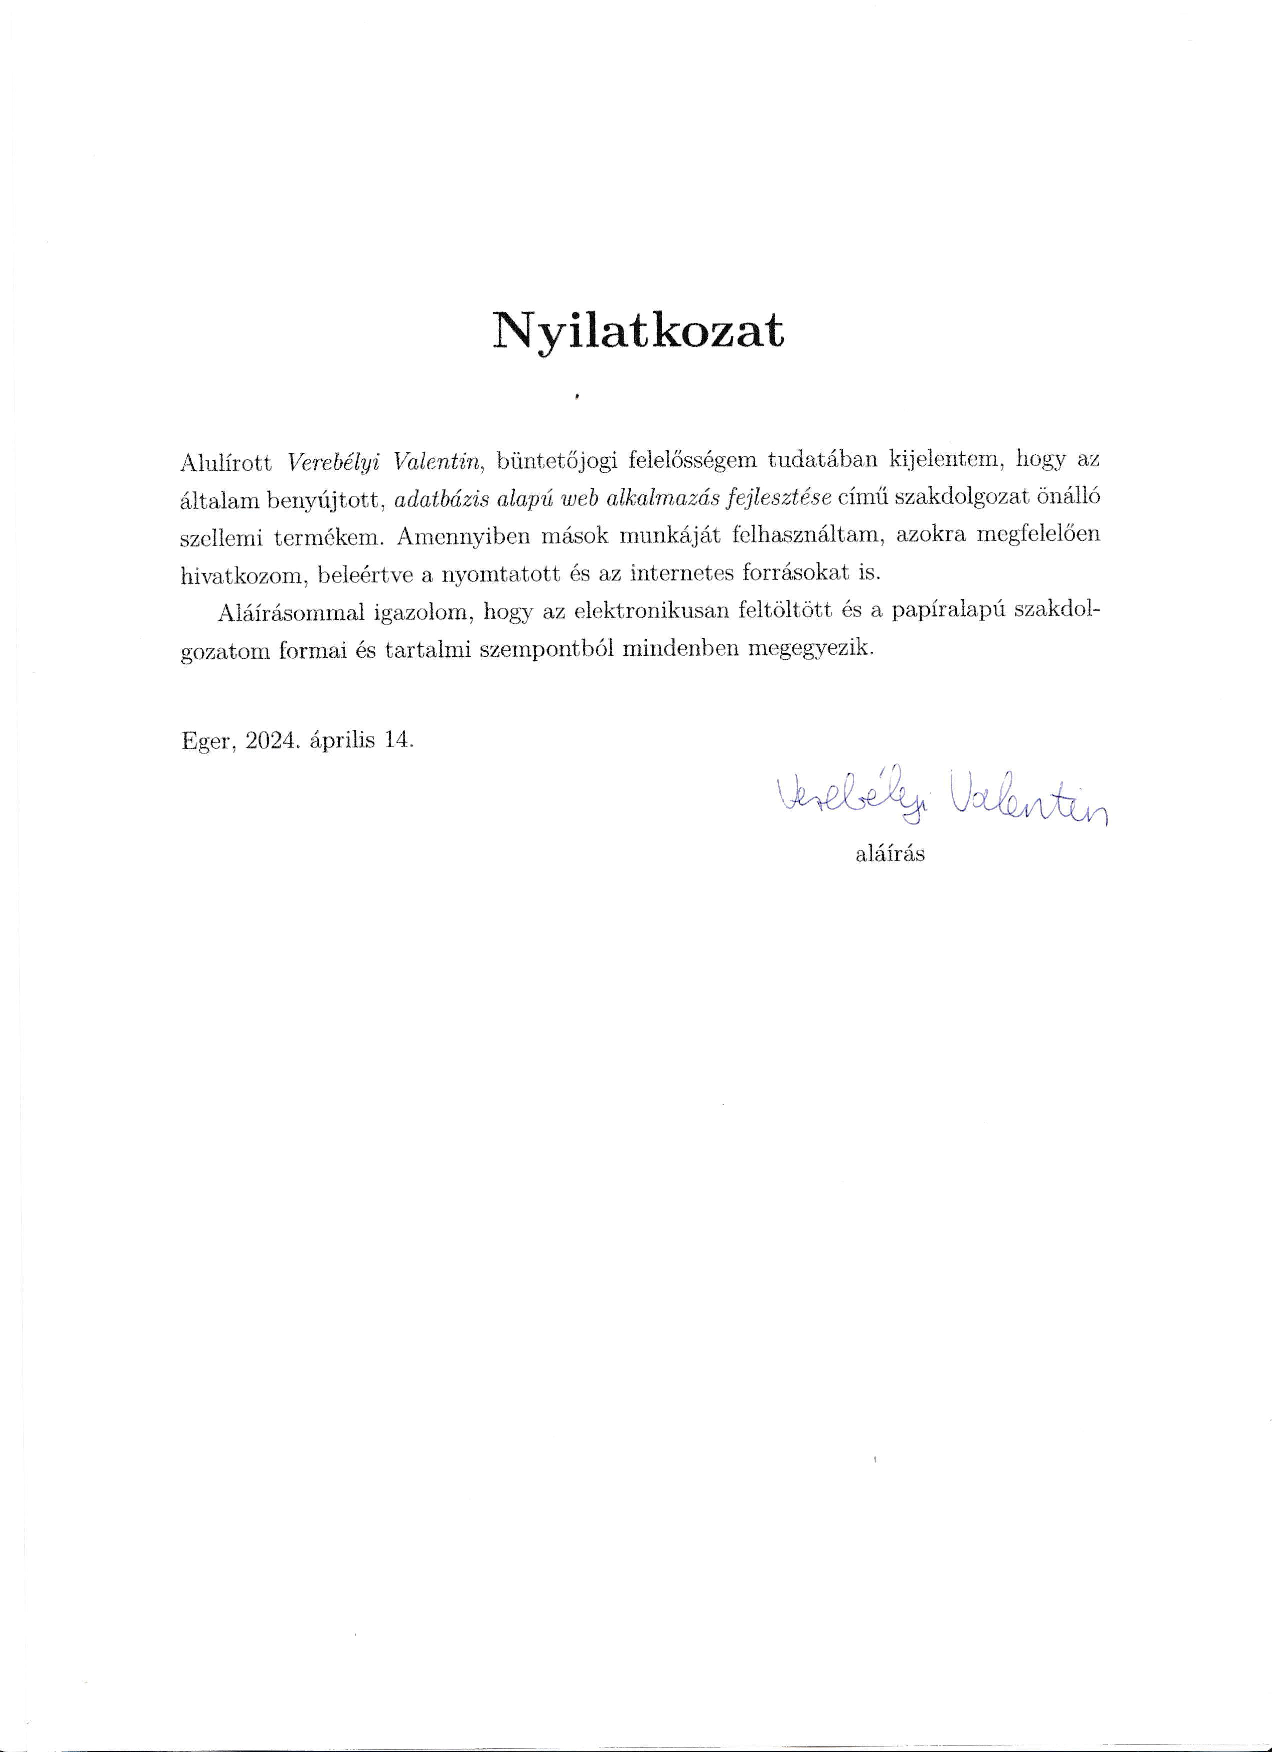
\includepdf{nyilatkozat.pdf}
\end{document}